%
% Qucs Test Report: SPICE to Qucs conversion: Test File 1
%
% Copyright (C) 2007 Mike Brinson <mbrin72043@yahoo.co.uk>
%
% Permission is granted to copy, distribute and/or modify this document
% under the terms of the GNU Free Documentation License, Version 1.1
% or any later version published by the Free Software Foundation.
%

% redefine subfigure caption
\renewcommand{\thesubfigure}{\thefigure(\alph{subfigure})}
\makeatletter
  \renewcommand{\@thesubfigure}{\thesubfigure:\space}
  \renewcommand{\p@subfigure}{}
\makeatother

% redefine subtable caption
\renewcommand{\thesubtable}{\thetable(\alph{subtable})}
\makeatletter
  \renewcommand{\@thesubtable}{\thesubtable:\space}
  \renewcommand{\p@subtable}{}
\makeatother

\tutsection{Introduction}
\tutsubsection{Title}
DC and independent voltage pulse generator test.
\tutsubsection{Test file name}

\tutsubsection{SPICE specification}

Format:
\linebreak 
\bigskip 
\begin{footnotesize}\textbf{VX N+ N- [[DC]  DC/TRAN VALUE]  [AC [ACMAG [ACPHASE]]]}                                                         \end{footnotesize}

Notes: 
\begin{enumerate}
 \item Characters [ and ] enclose optional items
 \item Character / denotes OR
 \item Independent voltage source names begin with the letter V
 \item X denotes name of source
 \item N+ and N- are the positive and negative nodes respectively
 \item Voltage sources need not be grounded
\end{enumerate}

\begin{flushleft}
Specification of SPICE statement being tested:                                              \end{flushleft}


VX N+ N- [[DC] VALUE] [PULSE(V1 V2 [ TD [ TR [ TF [ PW [PER]]]]]]
\vspace{4mm}
Notes:
\begin{enumerate}
 \item PULSE generates a periodic pulse, where
 \item V1 is the initial value; default: must be specified
 \item V2 is the pulsed value; default: must be specified
 \item TD is the delay time; default value = TSTEP
 \item TR is the rise time; default value = TSTEP
 \item TF is the fall time; default value = TSTEP
 \item PW is the pulse width; default value = TSTOP
 \item PER is the period; default value = TSTOP
\end{enumerate}




\tutsection{Test code and schematic}

SPICE code: File \verb|S2Q_test1.cir|

\begin{lstlisting}[
 language=Clean, 
 basicstyle=\small]

* SPICE to Qucs syntax test file 1.
* DC and independent voltage pulse sources, plus resistors.
*
.subckt S2Q_test1 p01 p02 p03 p04 p05 p06 p07 p08 p09 p10 p11
v1 p01 0 1v
r1 p01 0 10k
*
v2 p02 0 dc 1v
r2 p02 0 10k
*
v3 p03 0 pulse(0 5)
r3 p03 0 10k
*
v4 p04 0 pulse( 0 5 20n)
r4 p04 0 10k
*
v5 p05 0 pulse(0 5 20n 10n)
r5 p05 0 10k
*
v6 p06 0 pulse(0 5 20n 10n 10n)
r6 p06 0 10k
*
v7 p07 0 pulse(0 5 20n 10n 10n 50n)
r7 p07 0 10k
*
v8 p08 0 pulse(0 5 20n 10n 10n 50n 100n)
r8 p08 0 10k
*
v9 p09 0 pulse(0 5 20n 1n 1n 20n 40n)
r9 p09 0 10k
*
v10 p10 0 pulse(0 5 20n 0.1n 0.1n 5n 50n)
r10 p10 0 10k
*
v11 p11 0 dc 5v pulse(0 5 20n 0.5n 0.5n 10n 20n)
r11 p11 0 10k
.ends
.end
\end{lstlisting}


\begin{figure}
  \centering
  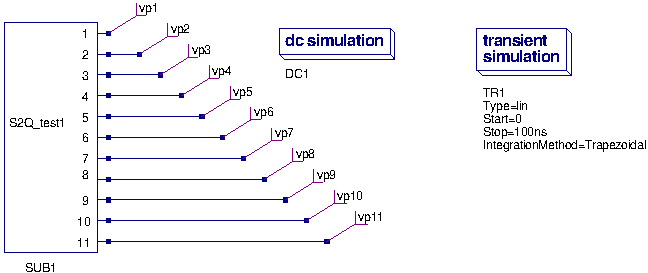
\includegraphics[width=0.9\linewidth]{S2Q_test1_sch}
  \caption{SPICE to Qucs conversion: Test1}
  \label{fig:S2Qtest1_1}
\end{figure} 

\tutsection{History of simulation results}
\tutsubsection{March 8 2007, Simulation tests by Mike Brinson}
\begin{enumerate}
 \item Test 1  : Vp1.Vt;  Pass correct result.
 \item Test 2  : Vp2.Vt;  Pass correct result.
 \item Test 3  : Vp3.Vt;  \textbf{Fail} TR and TF should default to TSTEP [TSTEP=1nS in test]
 \item Test 4  : Vp4.Vt; \textbf{ Fail} TR and TF should default to TSTEP [TSTEP=1nS in test]
 \item Test 5  : Vp5.Vt;  Pass.
 \item Test 6  : Vp6.Vt;  Pass.
 \item Test 7  : Vp7.Vt;  Pass.
 \item Test 8  : Vp8.Vt;  Pass.
 \item Test 9  : Vp9.Vt;  \textbf{Fail} - waveform should repeat after 60ns.
 \item Test 10 : Vp10.Vt; \textbf{Fail} - waveform should repeat after 70ns.
 \item \begin{flushleft}
Test 11 : Vp11.Vt;\textbf{ Fail} \end{flushleft}
\begin{flushleft}
 \hspace*{5mm} 1. waveform should repeat after 40ns, 
				\linebreak 
 \hspace*{5mm} 2. \verb|Vdc:V11 _cnet8 _ref U="0"| incorrect, 


 \hspace*{11mm}should be \verb|Vdc:V11 _cnet8 _ref U="5"|                                                                                                         \end{flushleft}
\end{enumerate}


\begin{figure}
  \centering
\begin{lstlisting}[
 language=Clean, 
 basicstyle=\scriptsize]
# Qucs 0.0.11  /media/hda2/spice_to_qucs_prj/s2Q(test1).sch

.Def:S2Q_test1 _net0 _net1 _net2 _net3 _net4 _net5 _net6 
               _net7 _net8 _net9 _net10
Sub:X1 _net0 _net1 _net2 _net3 _net4 _net5 _net6 _net7 
               _net8 _net9 _net10 gnd Type="S2Q_test1_cir"
.Def:End

.Def:S2Q_test1_cir _netP01 _netP02 _netP03 _netP04 _netP05 
               _netP06 _netP07 _netP08 _netP09 _netP10 _netP11 _ref
  .Def:S2Q_TEST1 _ref _netP01 _netP02 _netP03 _netP04 _netP05 
               _netP06 _netP07 _netP08 _netP09 _netP10 _netP11
  Vpulse:V11 _netP11 _cnet8 U1="0" U2="5" T1="20n" 
               Tr="0.5n" Tf="0.5n" T2="3.1e-08"
  Vpulse:V10 _netP10 _cnet7 U1="0" U2="5" T1="20n" 
               Tr="0.1n" Tf="0.1n" T2="2.52e-08"
  Vpulse:V9 _netP09 _cnet6 U1="0" U2="5" T1="20n" 
               Tr="1n" Tf="1n" T2="4.2e-08"
  Vpulse:V8 _netP08 _cnet5 U1="0" U2="5" T1="20n" 
               Tr="10n" Tf="10n" T2="9e-08"
  Vpulse:V7 _netP07 _cnet4 U1="0" U2="5" T1="20n" 
               Tr="10n" Tf="10n" T2="9e-08"
  Vpulse:V6 _netP06 _cnet3 U1="0" U2="5" T1="20n" 
               Tr="10n" Tf="10n" T2="4e-08"
  Vpulse:V5 _netP05 _cnet2 U1="0" U2="5" 
               T1="20n" Tr="10n" T2="3e-08"
  Vpulse:V4 _netP04 _cnet1 U1="0" U2="5" 
               T1="20n" T2="2e-08"
  Vpulse:V3 _netP03 _cnet0 U1="0" 
               U2="5" T2="0" T1="0"
  Vdc:V1 _netP01 _ref U="1V"
  R:R1 _netP01 _ref R="10k"
  Vdc:V2 _netP02 _ref U="1V"
  R:R2 _netP02 _ref R="10k"
  Vdc:V3 _cnet0 _ref U="0"
  R:R3 _netP03 _ref R="10k"
  Vdc:V4 _cnet1 _ref U="0"
  R:R4 _netP04 _ref R="10k"
  Vdc:V5 _cnet2 _ref U="0"
  R:R5 _netP05 _ref R="10k"
  Vdc:V6 _cnet3 _ref U="0"
  R:R6 _netP06 _ref R="10k"
  Vdc:V7 _cnet4 _ref U="0"
  R:R7 _netP07 _ref R="10k"
  Vdc:V8 _cnet5 _ref U="0"
  R:R8 _netP08 _ref R="10k"
  Vdc:V9 _cnet6 _ref U="0"
  R:R9 _netP09 _ref R="10k"
  Vdc:V10 _cnet7 _ref U="0"
  R:R10 _netP10 _ref R="10k"
  Vdc:V11 _cnet8 _ref U="0"
  R:R11 _netP11 _ref R="10k"
  .Def:End
  Sub:X1 _ref _netP01 _netP02 _netP03 _netP04 _netP05 
         _netP06 _netP07 _netP08 _netP09 _netP10 _netP11 Type="S2Q_TEST1"
.Def:End


.DC:DC1 Temp="26.85" reltol="0.001" abstol="1 pA" vntol="1 uV" 
saveOPs="no" MaxIter="150" saveAll="no" convHelper="none" Solver="CroutLU"
Sub:SUB1 vp1 vp2 vp3 vp4 vp5 vp6 vp7 vp8 vp9 vp10 vp11 Type="S2Q_test1"
.TR:TR1 Type="lin" Start="0" Stop="100ns" Points="500" 
IntegrationMethod="Trapezoidal" Order="2" InitialStep="1 ns" 
MinStep="1e-16" MaxIter="150" reltol="0.001" abstol="1 pA"  
vntol="1 uV" Temp="26.85" LTEreltol="1e-3" LTEabstol="1e-6" LTEfactor="1" 
Solver="CroutLU" relaxTSR="no" initialDC="yes" MaxStep="0"

\end{lstlisting}
 \caption{Qucs netlist [Edited to fit on page width]}
  \label{fig:S2Qtest1_2}
\end{figure} 

\begin{figure}
  \centering
  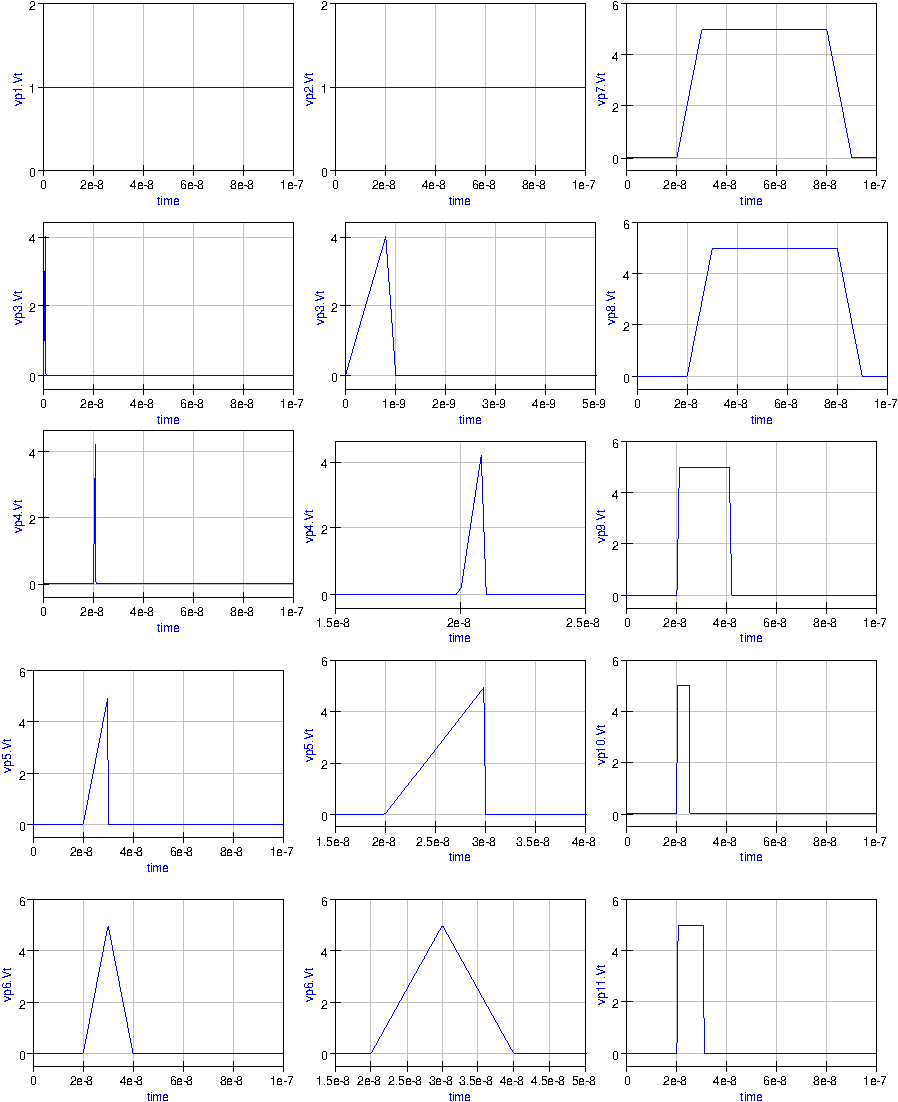
\includegraphics[width=0.9\linewidth]{S2Q_test1_dpl}
  \caption{SPICE to Qucs conversion: Test1 simulation waveforms}
  \label{fig:S2Qtest1_3} 
\end{figure} 



\tutsubsection{March 10 2007, Simulation tests by Mike Brinson}
Code modified   * \verb|check_spice.cpp|: Handling periodic pulse sources correctly. Also default Tr/Tf values for these sources to a given .TRAN step value : Stefan Jahn.

\vspace{5mm}
Restriction on SPICE code: $TD+TR+PW+TF < PER$, otherwise a negative TL time for the repetitive pulse occurs and simulation fails.

\vspace{5mm}
SPICE test file \verb|S2Q_test1.cir| modified: Mike Brinson
\vspace{5mm}
\begin{figure}
  \centering
\begin{lstlisting}[
 language=Clean, 
 basicstyle=\small]
* SPICE to Qucs syntax test file 1.
* DC and independent voltage pulse sources, plus resistors.
*
.subckt S2Q_test1 p01 p02 p03 p04 p05 p06 p07 p08 p09 p10 p11
v1 p01 0 1v
r1 p01 0 10k
*
v2 p02 0 dc 1v
r2 p02 0 10k
*
v3 p03 0 pulse(0 5)
r3 p03 0 10k
*
v4 p04 0 pulse( 0 5 20n)
r4 p04 0 10k
*
v5 p05 0 pulse(0 5 20n 10n)
r5 p05 0 10k
*
v6 p06 0 pulse(0 5 20n 10n 10n)
r6 p06 0 10k
*
v7 p07 0 pulse(0 5 20n 10n 10n 50n)
r7 p07 0 10k
*
v8 p08 0 pulse(0 5 20n 10n 10n 50n 100n)
r8 p08 0 10k
*
v9 p09 0 pulse(0 5 10n 1n 1n 20n 40n)
r9 p09 0 10k
*
v10 p10 0 pulse(0 5 20n 0.1n 0.1n 5n 50n)
r10 p10 0 10k
*
v11 p11 0 dc 5v pulse(-3 5 20n 0.5n 0.5n 10n 40n)
r11 p11 0 10k
.ends
.end
\end{lstlisting}
 \caption{Modified SPICE test1 netlist}
  \label{fig:S2Qtest1_4}
\end{figure} 


\begin{enumerate}
 \item Test 1  : Vp1.Vt;  Pass.
 \item Test 2  : Vp2.Vt;  Pass. 
 \item Test 3  : Vp3.Vt;  Pass
 \item Test 4  : Vp4.Vt;  Pass
 \item Test 5  : Vp5.Vt;  Pass.
 \item Test 6  : Vp6.Vt;  Pass.
 \item Test 7  : Vp7.Vt;  Pass.
 \item Test 8  : Vp8.Vt;  Pass.
 \item Test 9  : Vp9.Vt;  Pass.
 \item Test 10 : Vp10.Vt; Pass.
 \item \begin{flushleft}
Test 11 : Vp11.Vt; Pass \end{flushleft}
\end{enumerate}

\begin{figure}
  \centering
  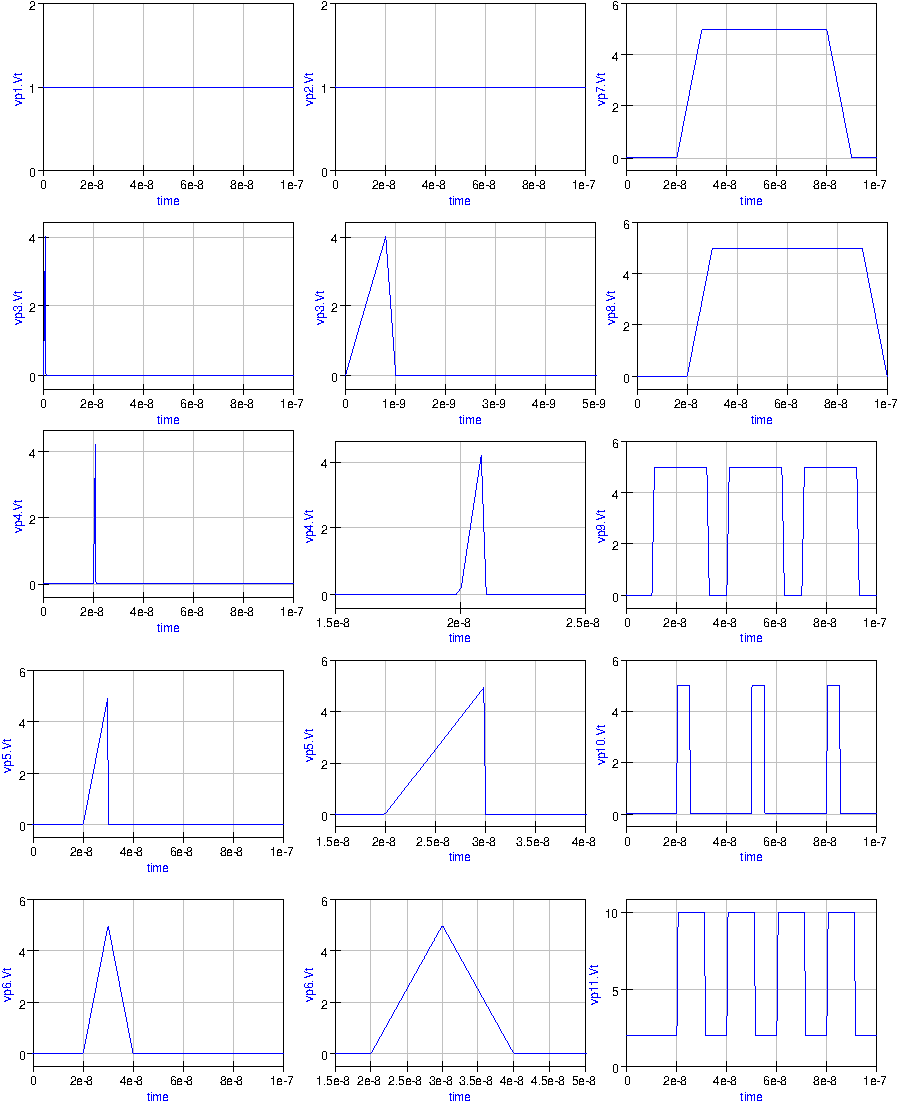
\includegraphics[width=0.9\linewidth]{S2Q_test1_mod_dpl}
  \caption{SPICE to Qucs conversion: Modified test1 simulation waveforms} 
  \label{fig:S2Qtest1_5} 
\end{figure} 

\begin{figure}
  \centering
\begin{lstlisting}[
 language=Clean, 
 basicstyle=\scriptsize]
# Qucs 0.0.11  /media/hda2/spice_to_qucs_prj/s2Q(test1).sch

.Def:S2Q_test1 _net0 _net5 _net1 _net6 _net2 _net7 _net3 
_net8 _net4 _net9 _net10
Sub:X1 _net0 _net5 _net1 _net6 _net2 _net7 _net3 _net8 
_net4 _net9 _net10 gnd Type="S2Q_test1_cir"
.Def:End

.Def:S2Q_test1_cir _netP01 _netP02 _netP03 _netP04 _netP05 
_netP06 _netP07 _netP08 _netP09 _netP10 _netP11 _ref
 .Def:S2Q_TEST1 _ref _netP01 _netP02 _netP03 _netP04 
_netP05 _netP06 _netP07 _netP08 _netP09 _netP10 _netP11
  Vrect:V11 _netP11 _cnet8 U="8" Td="20n" Tr="0.5n" Tf="0.5n" TH="1.1e-08" TL="9e-09"
  Vrect:V10 _netP10 _cnet7 U="5" Td="20n" Tr="0.1n" Tf="0.1n" TH="5.2e-09" TL="2.48e-08"
  Vrect:V9 _netP09 _cnet6 U="5" Td="10n" Tr="1n" Tf="1n" TH="2.2e-08" TL="8e-09"
  Vrect:V8 _netP08 _cnet5 U="5" Td="20n" Tr="10n" Tf="10n" TH="7e-08" TL="1e-08"
  Vpulse:V7 _netP07 _cnet4 U1="0" U2="5" T1="20n" Tr="10n" Tf="10n" T2="9e-08"
  Vpulse:V6 _netP06 _cnet3 U1="0" U2="5" T1="20n" Tr="10n" Tf="10n" T2="4e-08"
  Vpulse:V5 _netP05 _cnet2 U1="0" U2="5" T1="20n" Tr="10n" T2="3e-08"
  Vpulse:V4 _netP04 _cnet1 U1="0" U2="5" T1="20n" T2="2e-08"
  Vpulse:V3 _netP03 _cnet0 U1="0" U2="5" T2="0" T1="0"
  Vdc:V1 _netP01 _ref U="1V"
  R:R1 _netP01 _ref R="10k"
  Vdc:V2 _netP02 _ref U="1V"
  R:R2 _netP02 _ref R="10k"
  Vdc:V3 _cnet0 _ref U="0"
  R:R3 _netP03 _ref R="10k"
  Vdc:V4 _cnet1 _ref U="0"
  R:R4 _netP04 _ref R="10k"
  Vdc:V5 _cnet2 _ref U="0"
  R:R5 _netP05 _ref R="10k"
  Vdc:V6 _cnet3 _ref U="0"
  R:R6 _netP06 _ref R="10k"
  Vdc:V7 _cnet4 _ref U="0"
  R:R7 _netP07 _ref R="10k"
  Vdc:V8 _cnet5 _ref U="0"
  R:R8 _netP08 _ref R="10k"
  Vdc:V9 _cnet6 _ref U="0"
  R:R9 _netP09 _ref R="10k"
  Vdc:V10 _cnet7 _ref U="0"
  R:R10 _netP10 _ref R="10k"
  Vdc:V11 _cnet8 _ref U="2"
  R:R11 _netP11 _ref R="10k"
  .Def:End
  Sub:X1 _ref _netP01 _netP02 _netP03 _netP04 _netP05 _netP06 
  _netP07 _netP08 _netP09 _netP10 _netP11 Type="S2Q_TEST1"
.Def:End


.DC:DC1 Temp="26.85" reltol="0.001" abstol="1 pA" vntol="1 uV" 
saveOPs="no" MaxIter="150" saveAll="no" convHelper="none" Solver="CroutLU"
.TR:TR1 Type="lin" Start="0" Stop="100ns" Points="500" 
IntegrationMethod="Trapezoidal" Order="2" InitialStep="1 ns" 
MinStep="1e-16" MaxIter="150" reltol="0.001" abstol="1 pA" 
vntol="1 uV" Temp="26.85" LTEreltol="1e-3" LTEabstol="1e-6" 
LTEfactor="1" Solver="CroutLU" relaxTSR="no" initialDC="yes" MaxStep="0"
Sub:SUB1 vp1 vp2 vp3 vp4 vp5 vp6 vp7 vp8 vp9 vp10 vp11 Type="S2Q_test1"

\end{lstlisting}
 \caption{Qucs netlist for modified test1 SPICE netlist [Edited to fit on page width]}
  \label{fig:S2Qtest1_6}
\end{figure} 


\tutsection{References}
\begin{enumerate}
 \item A. Vladimirescu, Kaihe Zhang, A.R. Newton, D.O Pederson A. Sangiovanni-Vincentelli, SPICE 2G User's Guide (10 Aug 1981), Department of Electrical Engineering and Computer Sciences, University of California, Berkeley, Ca., 94720.
\item B. Johnson, T. Quarles, A.R. Newton, P.O. Pederson, A.Sangiovanni-Vincentelli, SPICE3 Version 3f User's Manual (October 1972),  Department of Electrical Engineering and Computer Sciences, University of California, Berkeley, Ca., 94720.
\item Andrei Vladimirescu, THE SPICE book,1994, John Wiley and Sons. Inc., ISBN 0-471-609-26-9.
\end{enumerate}


